\chapter{Konvoi}
\TODO{Yves}
\section{Motivation}
Ein Verband von Fahrzeugen muss Hilfsgüter nach einer Naturkatastrophe im Konvoi über
eine Passstraße steuern. Um keine Menschen auf dem unsicheren Terrain zu gefährden, muss
ein führerloses Transportsystem eingesetzt werden, um die Güter zu den von der Außenwelt
abgeschnitten Menschen zu bringen. Doch leider ist ein Fahrzeug aus dem Konvoi gestohlen
worden, und es muss schnell aus Ersatzteilen ein Neues gebaut werden.

\begin{capfigure}[Konvoi]
	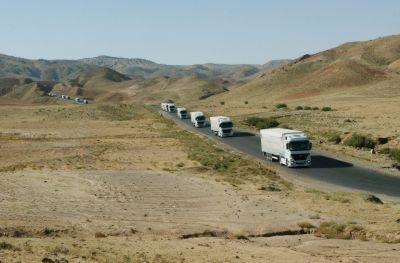
\includegraphics[width=\textwidth]{images/konvoi}
\end{capfigure}

\section{Aufgabenstellung}
Bauen Sie ein Fahrzeug aus den gegebenen Teilen, welches folgende Fähigkeiten hat:
\begin{itemize}
	\item Es soll einem vorgegebenen Pfad folgen, ohne ihn zu verlassen
	\item Es soll einen definierten Abstand zum führenden Fahrzeug einhalten
\end{itemize}

Achtung! Das Führungsfahrzeug wird bei jedem Transport je nach Gefahr den Pfad unterschiedlich
schnell entlang fahren

\begin{capfigure}[Strecke]
	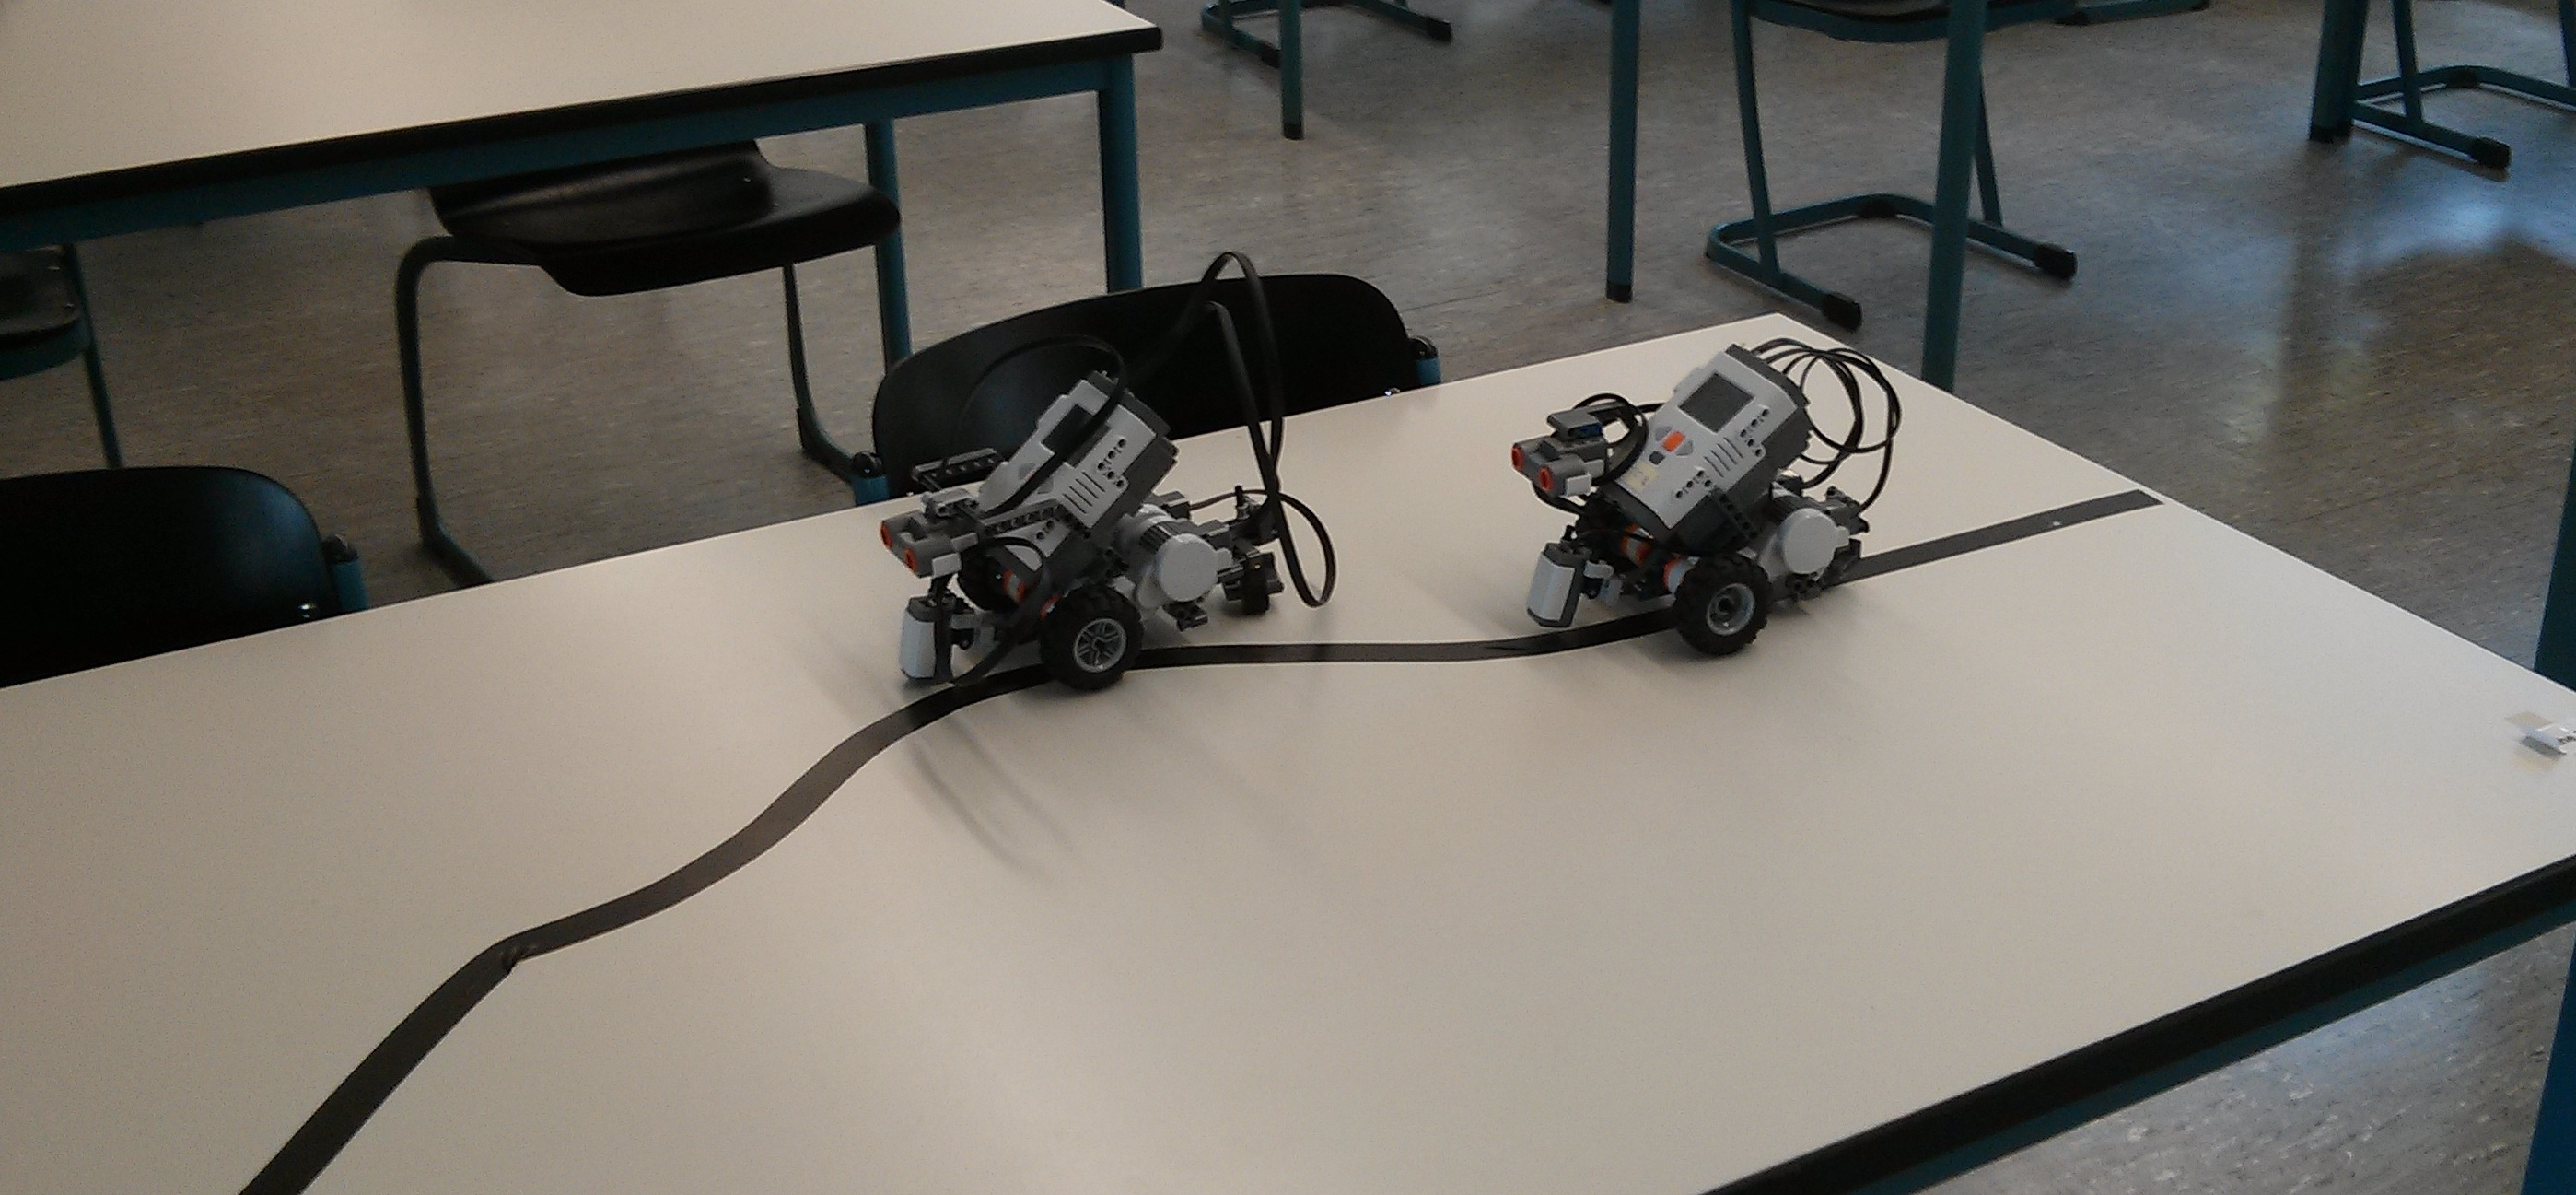
\includegraphics[width=\textwidth]{images/fotokonvoi}
\end{capfigure}
\section{Lösung}
Bei der Lösung haben wir uns dazu entschieden die Geschwindigkeit des Roboters in Abhängigkeit der Distanz zum vorfahrenden Roboters zu regulieren.

Der vorausfahrende Roboter reguliert seine Geschwindigkeit variabel.

Die Konstruktion ist für beide die des Standardlinienfolgers.

Die Lösung befindet sich auf der DVD unter \textit{Lösungen/Konvoi}.